\section{Classifier System}
\begin{frame}
    \frametitle{Classifier System}
    \begin{itemize}[<+->]
        \item Allows agent to learn
        \item Good Rules accumulate higher \emph{strength}
        \item Higher strength rules are more likely to win the bid and become the decision 
    \end{itemize}

    \vfill
    \pause
    The following slides are going to cover
    \begin{enumerate}[<+->]
        \item Encoding of CS and notations
        \item Evolution of strength
        \item Genetic algorithm
    \end{enumerate}
\end{frame}

\begin{frame}[allowframebreaks]
    \frametitle{Encodings for a classifier system}

    \begin{table}
        \begin{tabular}{llll}
            \hline
            \multicolumn{3}{l}{Code} & Meaning    \\ \hline
            1      & 0      & 0      & Good 1     \\
            0      & 1      & 0      & Good 2     \\
            0      & 0      & 1      & Good 3     \\
            0      & \#     & \#     & Not good 1 \\
            \#     & 0      & \#     & Not good 2 \\
            \#     & \#     & 0      & Not good 3 \\ \hline
            \end{tabular}
    \end{table}
    \vfill 
    1 : hold

    0: not hold

    \#: either

    \framebreak

    Define an exchange classifier
    \begin{center}
        Holding of $a$ + Holding of $\rho(a)$ + Trade / Not Trade
    \end{center}
    total of 3+3+1 codes
    \vfill
    \pause
    Define a comsumption classifier
    \begin{center}
        Holding of $a$ + Consume / Not Consume
    \end{center}

    \vfill
    \pause
    Denote $e=1,2,...E_a, c=1,2,...E_c$ index of the classifier system (for agent $a$).
    There will be total of $6\times 6 \times 2=72$ distinct classifiers.
\end{frame}

\begin{frame}
    \frametitle{Desicion Making}
    
    \setcounter{equation}{4}
    \begin{equation}
        M_e(z_{at}) = \{e : z_{at} \text{ matches the condition part of classifier } e\}
    \end{equation}



    Members of $\Me$ form a collection of potential "bidders".
    $e$ with the highest strength wins
    \begin{equation}
        \lambda_{at} = e_t(z_{at}) = \arg\max\{\Se : e \in \Me\}
    \end{equation}

    \pause

    Same for consumption desicion
    \begin{equation}
       \Mc = \{c : x_{at}^+ \text{ matches the condition part of classifier } c\}
    \end{equation}
    
    \begin{equation}
        \gamma_{at} = c_t(z_{at}) = \arg\max\{\Sc : c \in \Mc\}
    \end{equation}
    Along with the law of motion in Eq. \ref{eq:x-lom}
\end{frame}


\begin{frame}
    \frametitle{Evolution of Strength}
    \begin{equation}
        \tau^a_e(t) = 1 + \sum_{s=0}^t I^a_e(s)
    \end{equation}
    
    \newcommand{\tea}{\tau^a_e(t)}

    \begin{itemize}
        \item    $\tea$ : the count of successful trade using the classifier $e$ 
        up to time $t$. 
        \item  $I^a_e(t)$ : whether $e$ wins the auction (between classifiers) 
        and helps the agent successfully trade, i.e., $\lambda_{at} \cdot \lambda_{\rho_t(a)t} x_{\rho_t(a)t}=1$
    \end{itemize}

    \pause

    Analogously, 
    \begin{equation}
        \tau^a_c(t) = 1 + \sum_{s=0}^t I^a_c(s)
    \end{equation}
 
    \vfill 
    The strength of a classifier is a function of successful wins.
    \begin{align*}
        \Se &= S^a_{e \tau^a_e(t)} \\
        \Sc &= S^a_{c \tau^a_c(t)}
    \end{align*}
\end{frame}

\begin{frame}
    \frametitle{Bids}
    \begin{block}{Bid-paying Mechanism}
        Winning classifier $e^a_t$ pays its bids to the winning classifier $c^a_{t-1}$\\
        Winning classifier $c^a_t$ pays its bids to the winning classifier $e^a_t$
    \end{block}

    This mechanism rewards the former classifier that lead to its success, reinforcing the right decision.

    \pause
    The bid is set as $b_1(e)\Se$ for a exchange classifier, 
    and $b_2(c)\Sc$ for a consumption classifier.
    \begin{subequations}
        \begin{align}
            b_1(e) &= b_{11} + b_{12} \sigma_e \\
            b_2(c) &= b_{21} + b_{22} \sigma_c
        \end{align}
    \end{subequations}

    $\sigma_\cdot = \frac{1}{1+\text{number of \#'s in the classifier}}$. Higher uncertainty, lower bid.

\end{frame}

\begin{frame}[allowframebreaks]
    \frametitle{Evolution of Strength}

    \newcommand{\Setau}{S^a_{e \tau^a_e(t)}}
    \newcommand{\Setauf}{S^a_{e \tau^a_e(t)+1}}
    \newcommand{\Sctau}{S^a_{c \tau^a_c(t)}}
    \newcommand{\Sctaul}{S^a_{c \tau^a_c(t)-1}}
    \newcommand{\gct}{\gamma^a_{ct}}

    \begin{align}
        \begin{split}
            \Sctau =& \Sctaul - \frac{1}{\tau^a_c(t) - 1} \Biggl[
                (1+b_2(c))\Sctaul \\
                &- \sum_e I^a_e(t)b_1\Setau - U_a(\gamma^a_{ct})
            \Biggl]
        \end{split} \\[2em]
        \begin{split}
            \Setauf =& \Setau - \frac{1}{\tau^a_e(t)} \Biggl[
                (1+b_1(e))\Setau \\
                &- \sum_c I^a_c(t)b_c \Sctau 
            \Biggl]
        \end{split}
    \end{align}
    
    The external payoff after making consumption desicion
    \begin{equation}
        U_a(\gct) = \gct\left[u_i(x_{at}^+) - s(f(a))\right] + (1-\gct)s(x_{at}^+)
    \end{equation}
    \begin{alertblock}{Possible Typo}
        I think the authors might have a typo here. $(1-\gct)s(x_{at}^+)$ 
        should be a minus since it is the cost of holding.
    \end{alertblock}
    \framebreak

    \begin{itemize}
        \item $\Setau$ and $\Sctau$ evolves recursively
        \item Average of past payoff (External reward + bid from other classifier)
        \item minus payment (bids made to other classifier)
        \item Only winning classifier pays the bid (the sum term)
        \item Indexing with counter $\tau_{(\cdot)}^a(t)$ : change is made only when successfully winning the auction.
    \end{itemize}
\end{frame}

\begin{frame}[plain]
    \begin{figure}
        \centering
        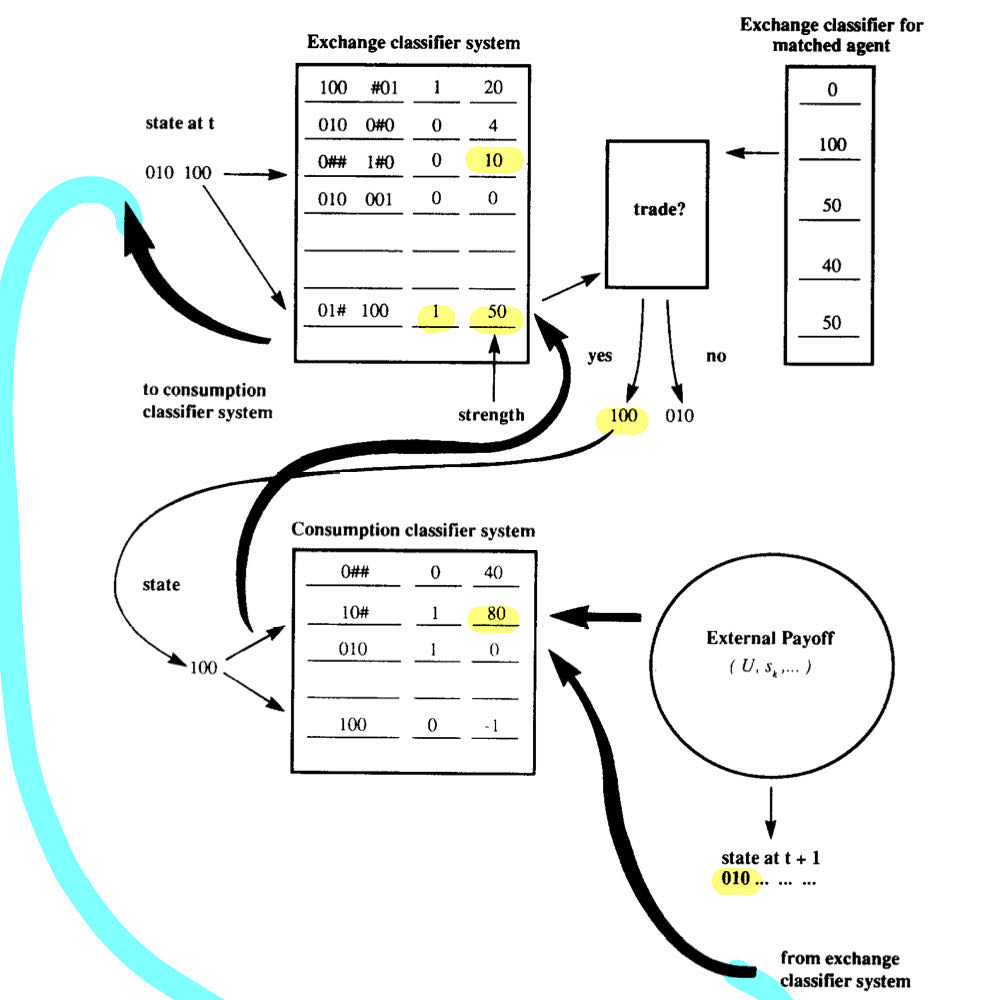
\includegraphics[height=\textheight]{img/Fig1_flow.jpg}
    \end{figure}
\end{frame}